\chapter{Super-cells and nanoislands}
\section{Simple}
This is the simplest super-cell to implement, it is just a n-replication of the unit cell along the lattice vectors.
%~~~~~~~~~~~~~~~~~~~~~~~~~~ FIGURE ~~~~~~~~~~~~~~~~~~~~~~~~~%
\begin{figure}[h!]
\centering
   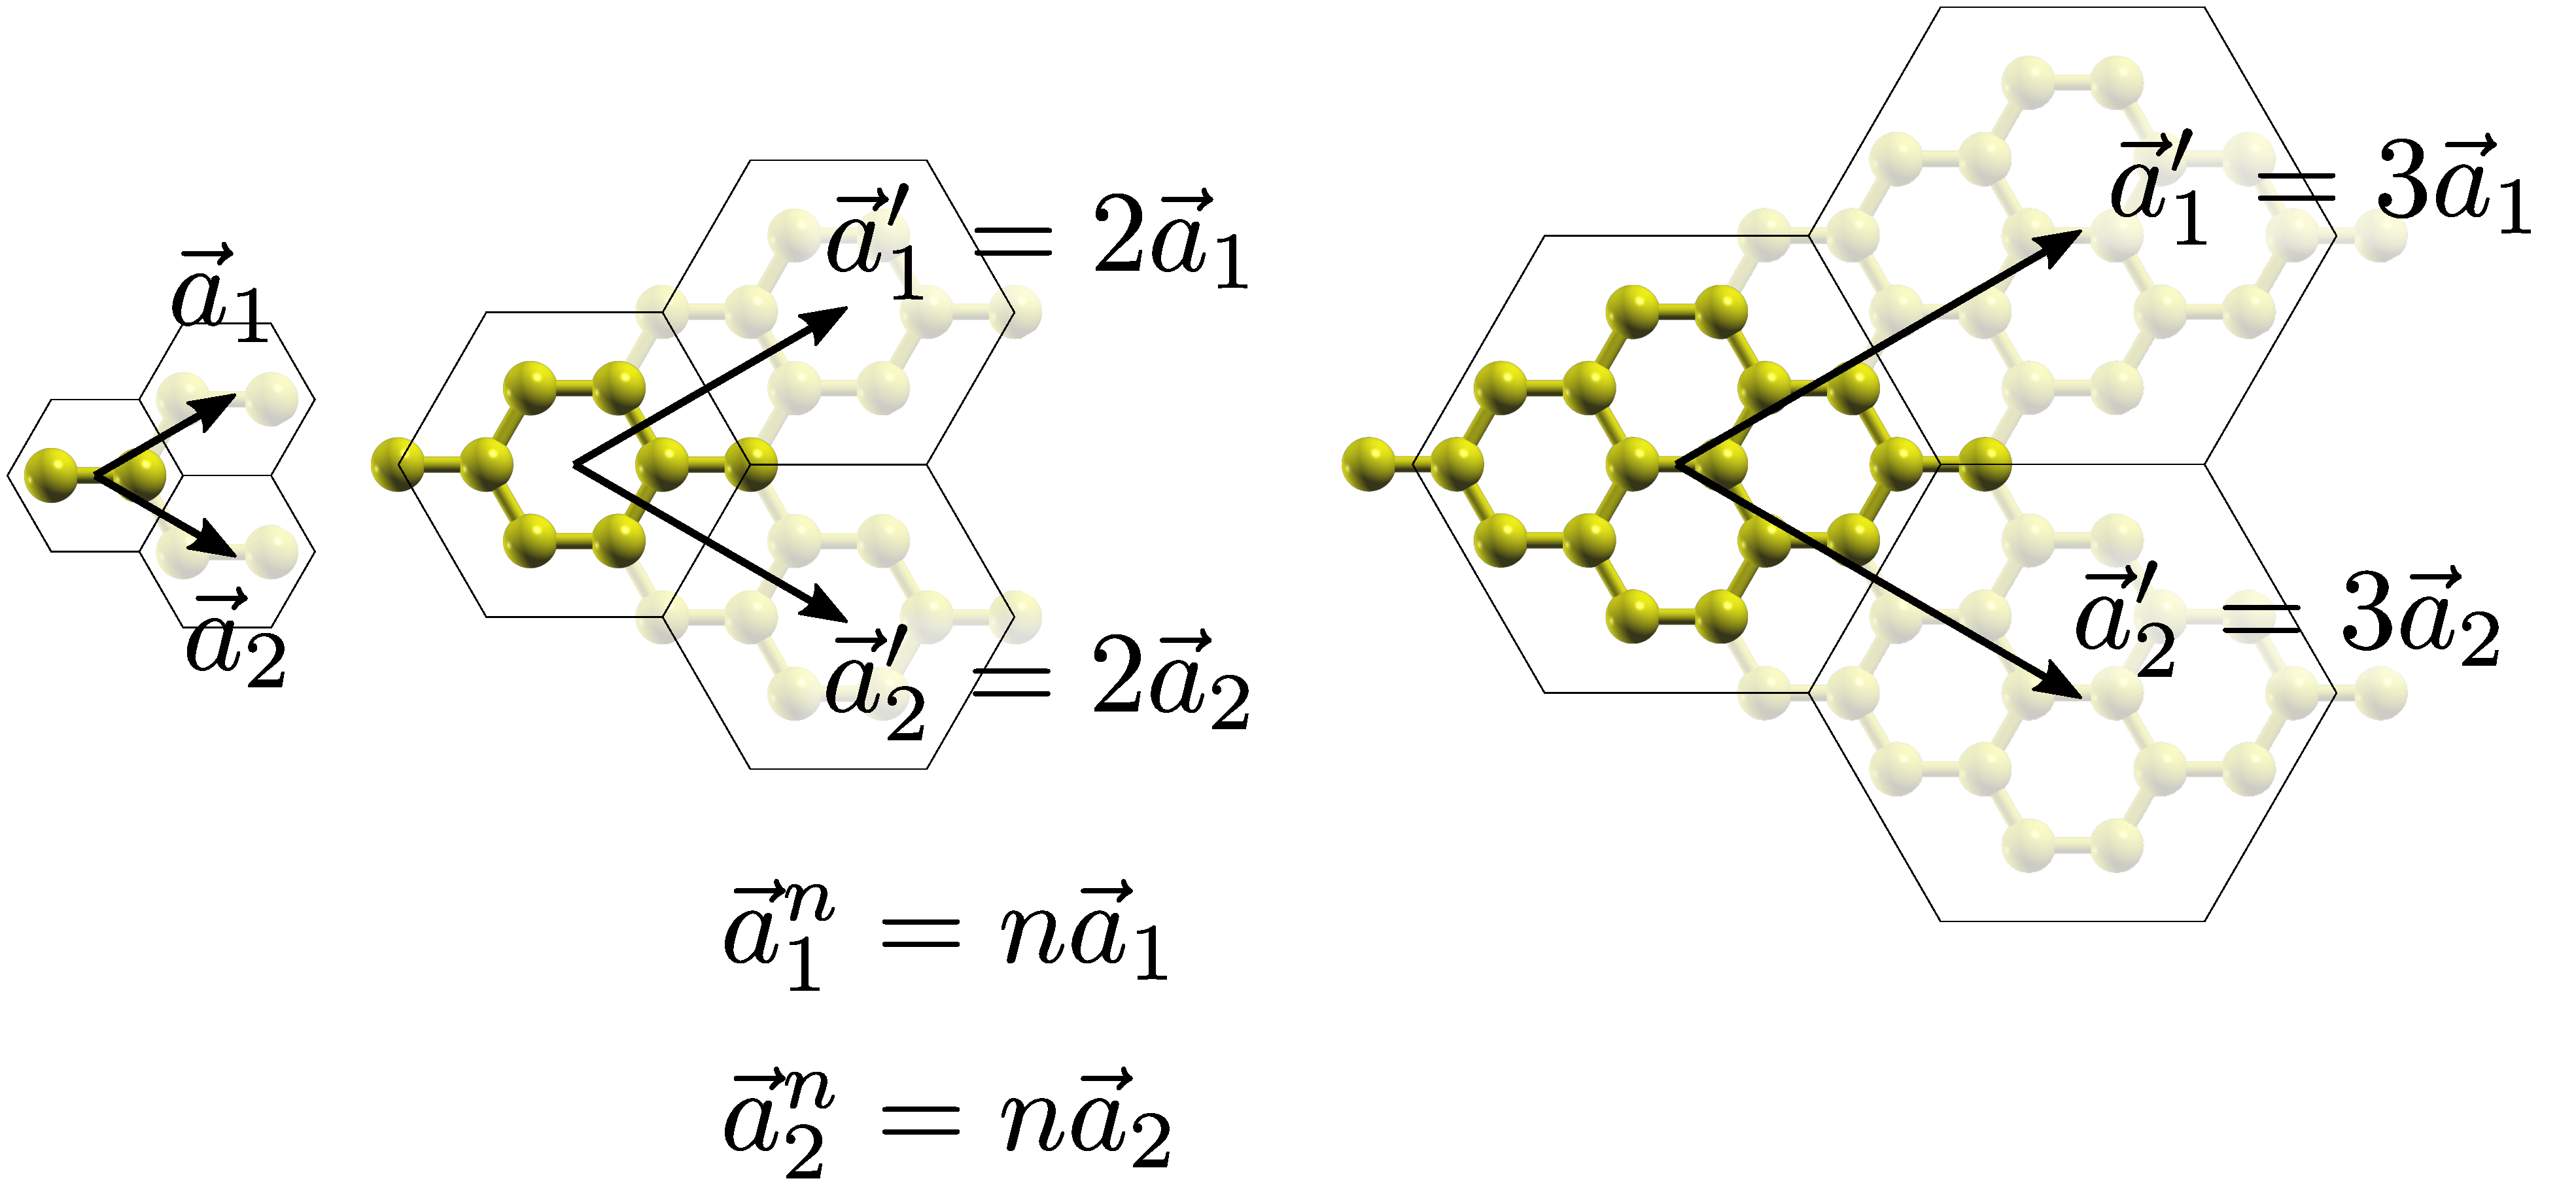
\includegraphics[width=0.8\textwidth]{appendix/figures/cells_simple.pdf}
\vspace{-5pt}
\caption{Caption}
\label{Label}
\end{figure}
\FloatBarrier
%~~~~~~~~~~~~~~~~~~~~~~~~~~~~~~~~~~~~~~~~~~~~~~~~~~~~~~~~~~~%
\begin{equation}
   N = 2n^2
\end{equation}


\section{Armchair}
Taking a Benzene ring as building block, one can replicate it in the proper positions in order to generate bigger and bigger armchair islands. The process is not straight forward since it is not enough to replicate along the lattice vectors (or $\pm$ combinations of them), but rather 
%~~~~~~~~~~~~~~~~~~~~~~~~~~ FIGURE ~~~~~~~~~~~~~~~~~~~~~~~~~%
\begin{figure}[h!]
\centering
   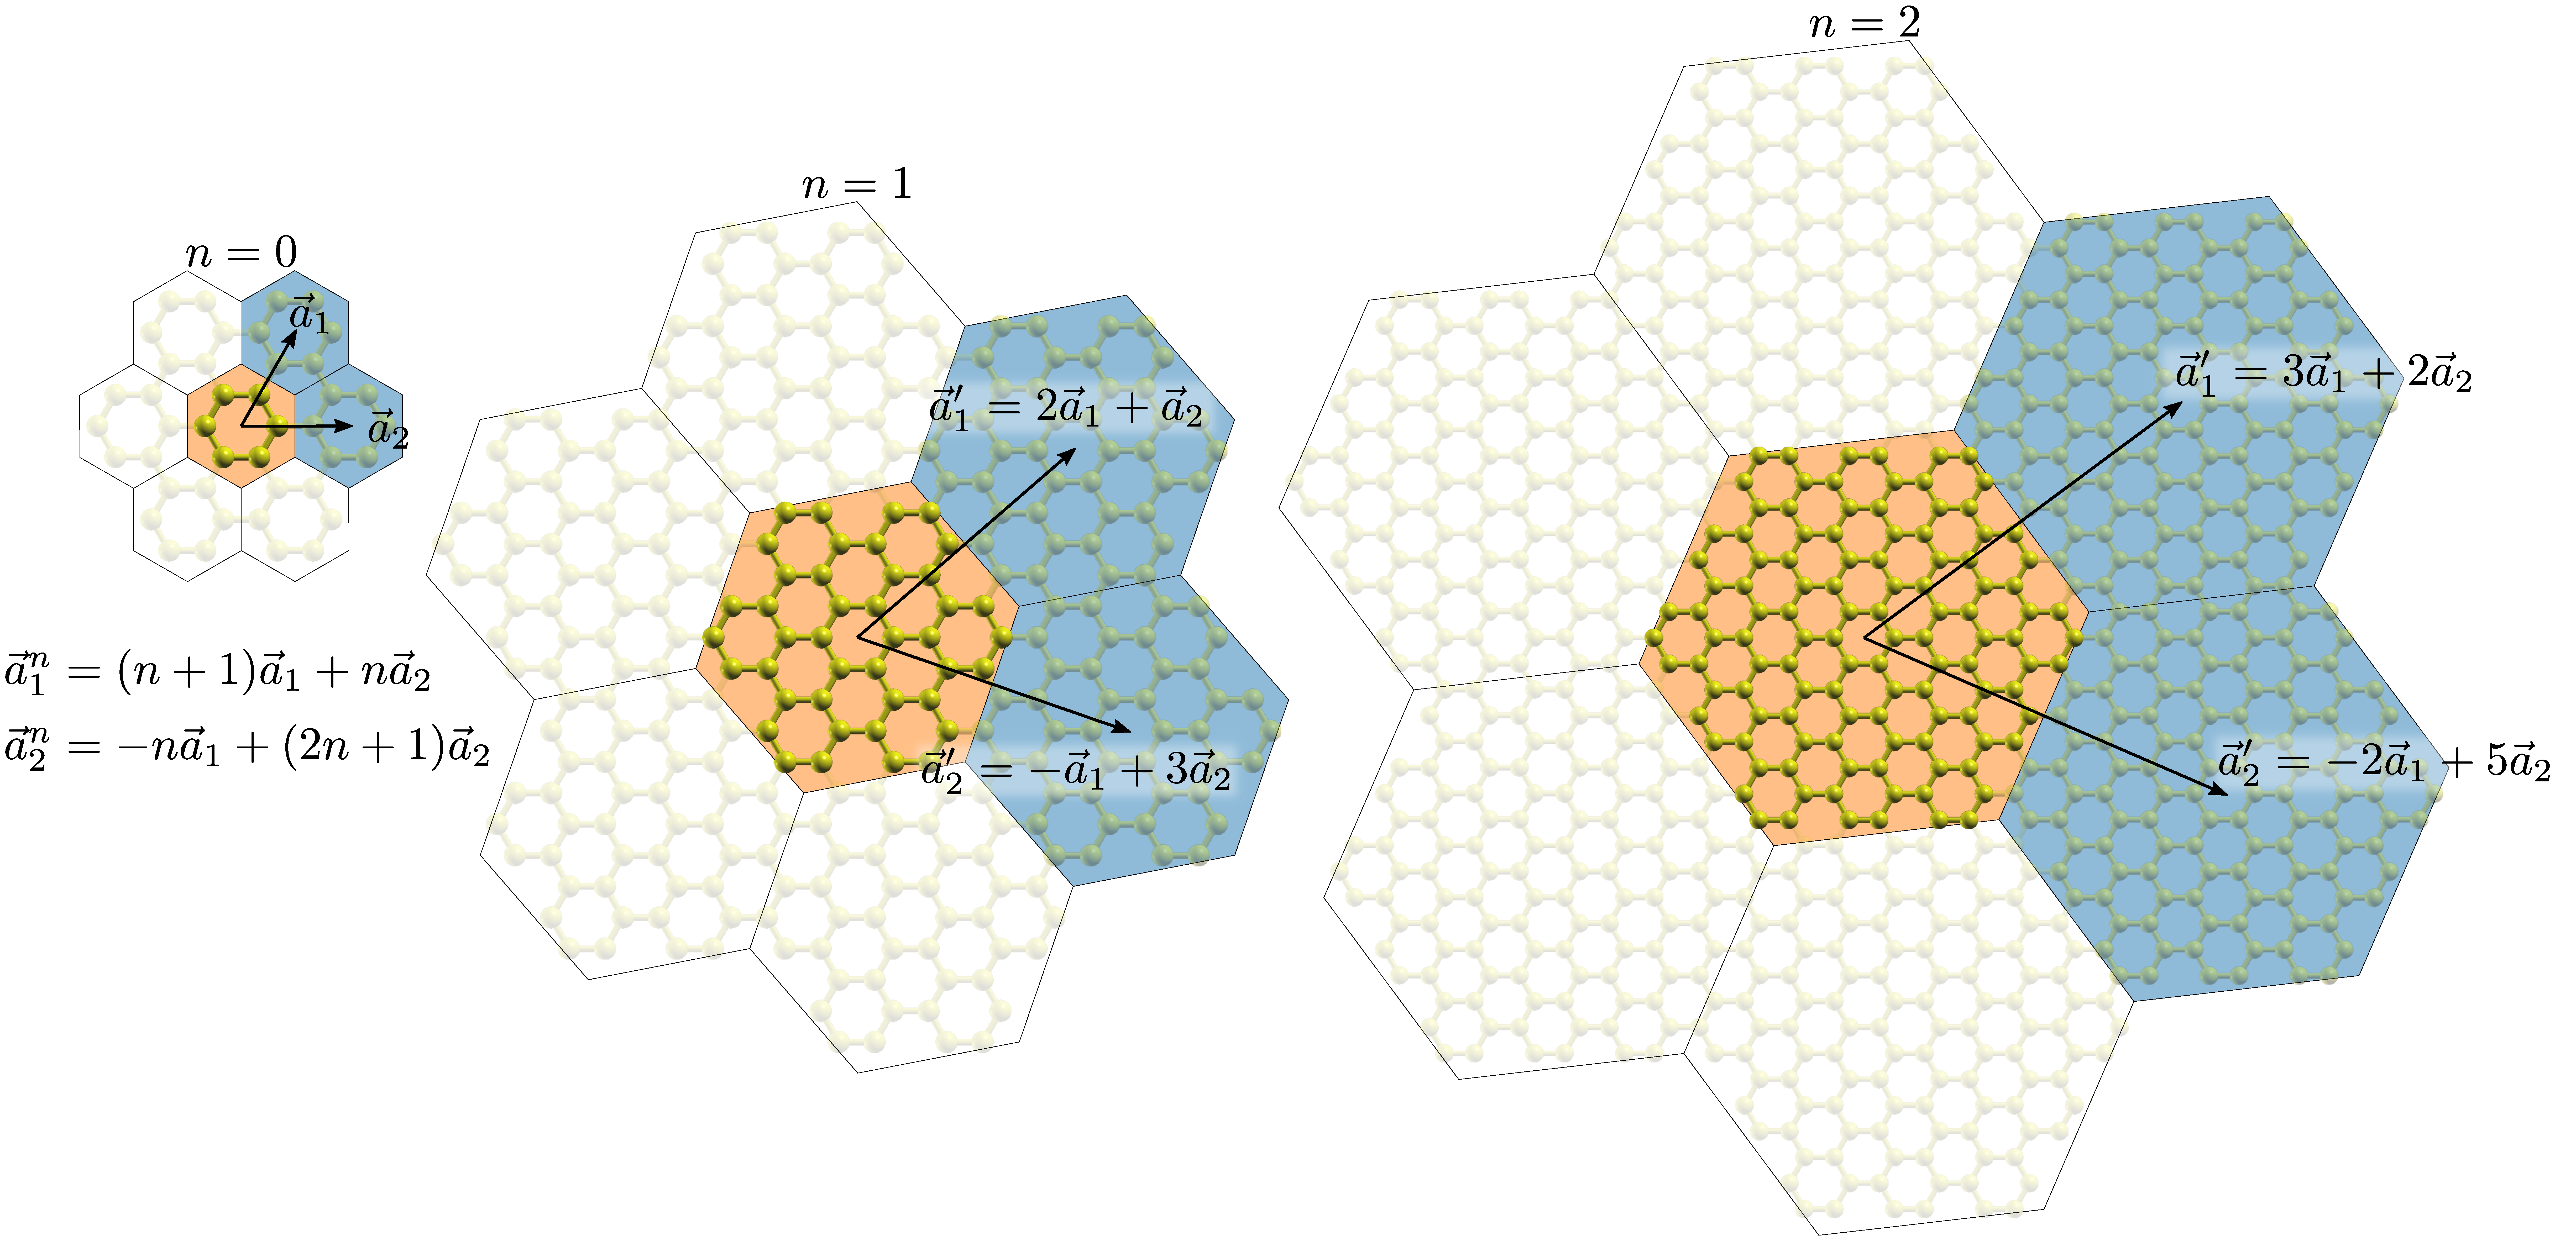
\includegraphics[width=0.8\textwidth]{appendix/figures/cells_ac.pdf}
\vspace{-5pt}
\caption{Caption}
\label{Label}
\end{figure}
\FloatBarrier
%~~~~~~~~~~~~~~~~~~~~~~~~~~~~~~~~~~~~~~~~~~~~~~~~~~~~~~~~~~~%
\begin{equation}
   N = 6\cdot(3n^2-3n+1)
\end{equation}

This is how fast the number of carbon atoms gros for the different kind of islands.

%~~~~~~~~~~~~~~~~~~~~~~~~~~ FIGURE ~~~~~~~~~~~~~~~~~~~~~~~~~%
\begin{figure}[h!]
\centering
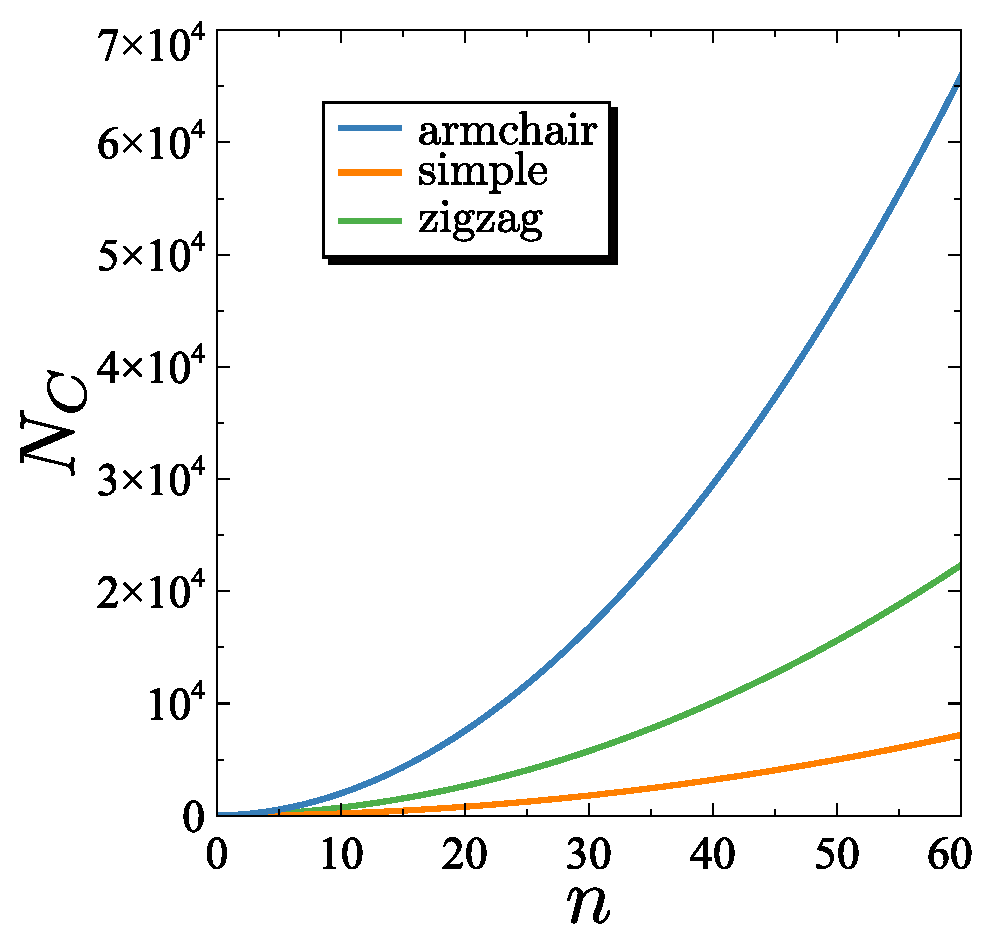
\includegraphics{appendix/figures/Nats.pdf}
\vspace{-5pt}
\caption{Caption}
\label{Label}
\end{figure}
\FloatBarrier
%~~~~~~~~~~~~~~~~~~~~~~~~~~~~~~~~~~~~~~~~~~~~~~~~~~~~~~~~~~~%
